\section{SMU HPC Clusters}

\begin{frame}{ManeFrame II (M2) Node Types}
\begin{table}
\tiny
\begin{tabular}{lllll}
\toprule
Type & Quantity & Cores & Memory [GB] & Additional Resources\\
\midrule
Standard-Memory & 176 & 36 & 256 & \\
Medium-Memory-1 & 35 & 36 & 768 & \\
Medium-Memory-2 & 4 & 24 & 768 & 3 TB SSD local scratch\\
High-Memory-1 & 5 & 36 & 1,536 & \\
High-Memory-2 & 6 & 40 & 1,536 & 3 TB SSD local scratch\\
GPGPU-1 & 36 & 36 & 256 & NVIDIA P100 GPU has 3,584 CUDA cores and 16 GB CoWoS\\
MIC-1 & 36 & 64 & 384 & 16 GB of high bandwidth (400 GB/s) stacked memory\\
VDI & 5 & 36 & 256 & NVIDIA Quadro M5000 GPU\\
v100x8 & 3 & 36 & 768 & 8 NVIDIA V100 GPUs with 5,120 CUDA cores and 32 GB CoWoS\\
Faculty Partner Nodes & 3 &  &  & Various research specific NVIDIA GPU configurations\\
\midrule
ManeFrame II & 354 & 11,276 & 120 TB & 2.8 PB storage and InfiniBand network\\
\bottomrule
\end{tabular}
\end{table}
\end{frame}

\begin{frame}{NVIDIA DGX SuperPOD (MP)}
\begin{columns}
\begin{column}{0.5\textwidth}
\begin{itemize}
\item 20 NVIDIA DGX nodes
\item 8 NVIDIA A100 80 GB GPUs per node
\item Dual AMD Epyc 7742 2.25 GHz 64-core ``Rome'' processors per node
\item 200 Gb/s \(\times\) 10 NVIDIA/Mellanox InfiniBand networking
\end{itemize}
\end{column}
\begin{column}{0.5\textwidth}
\begin{center}
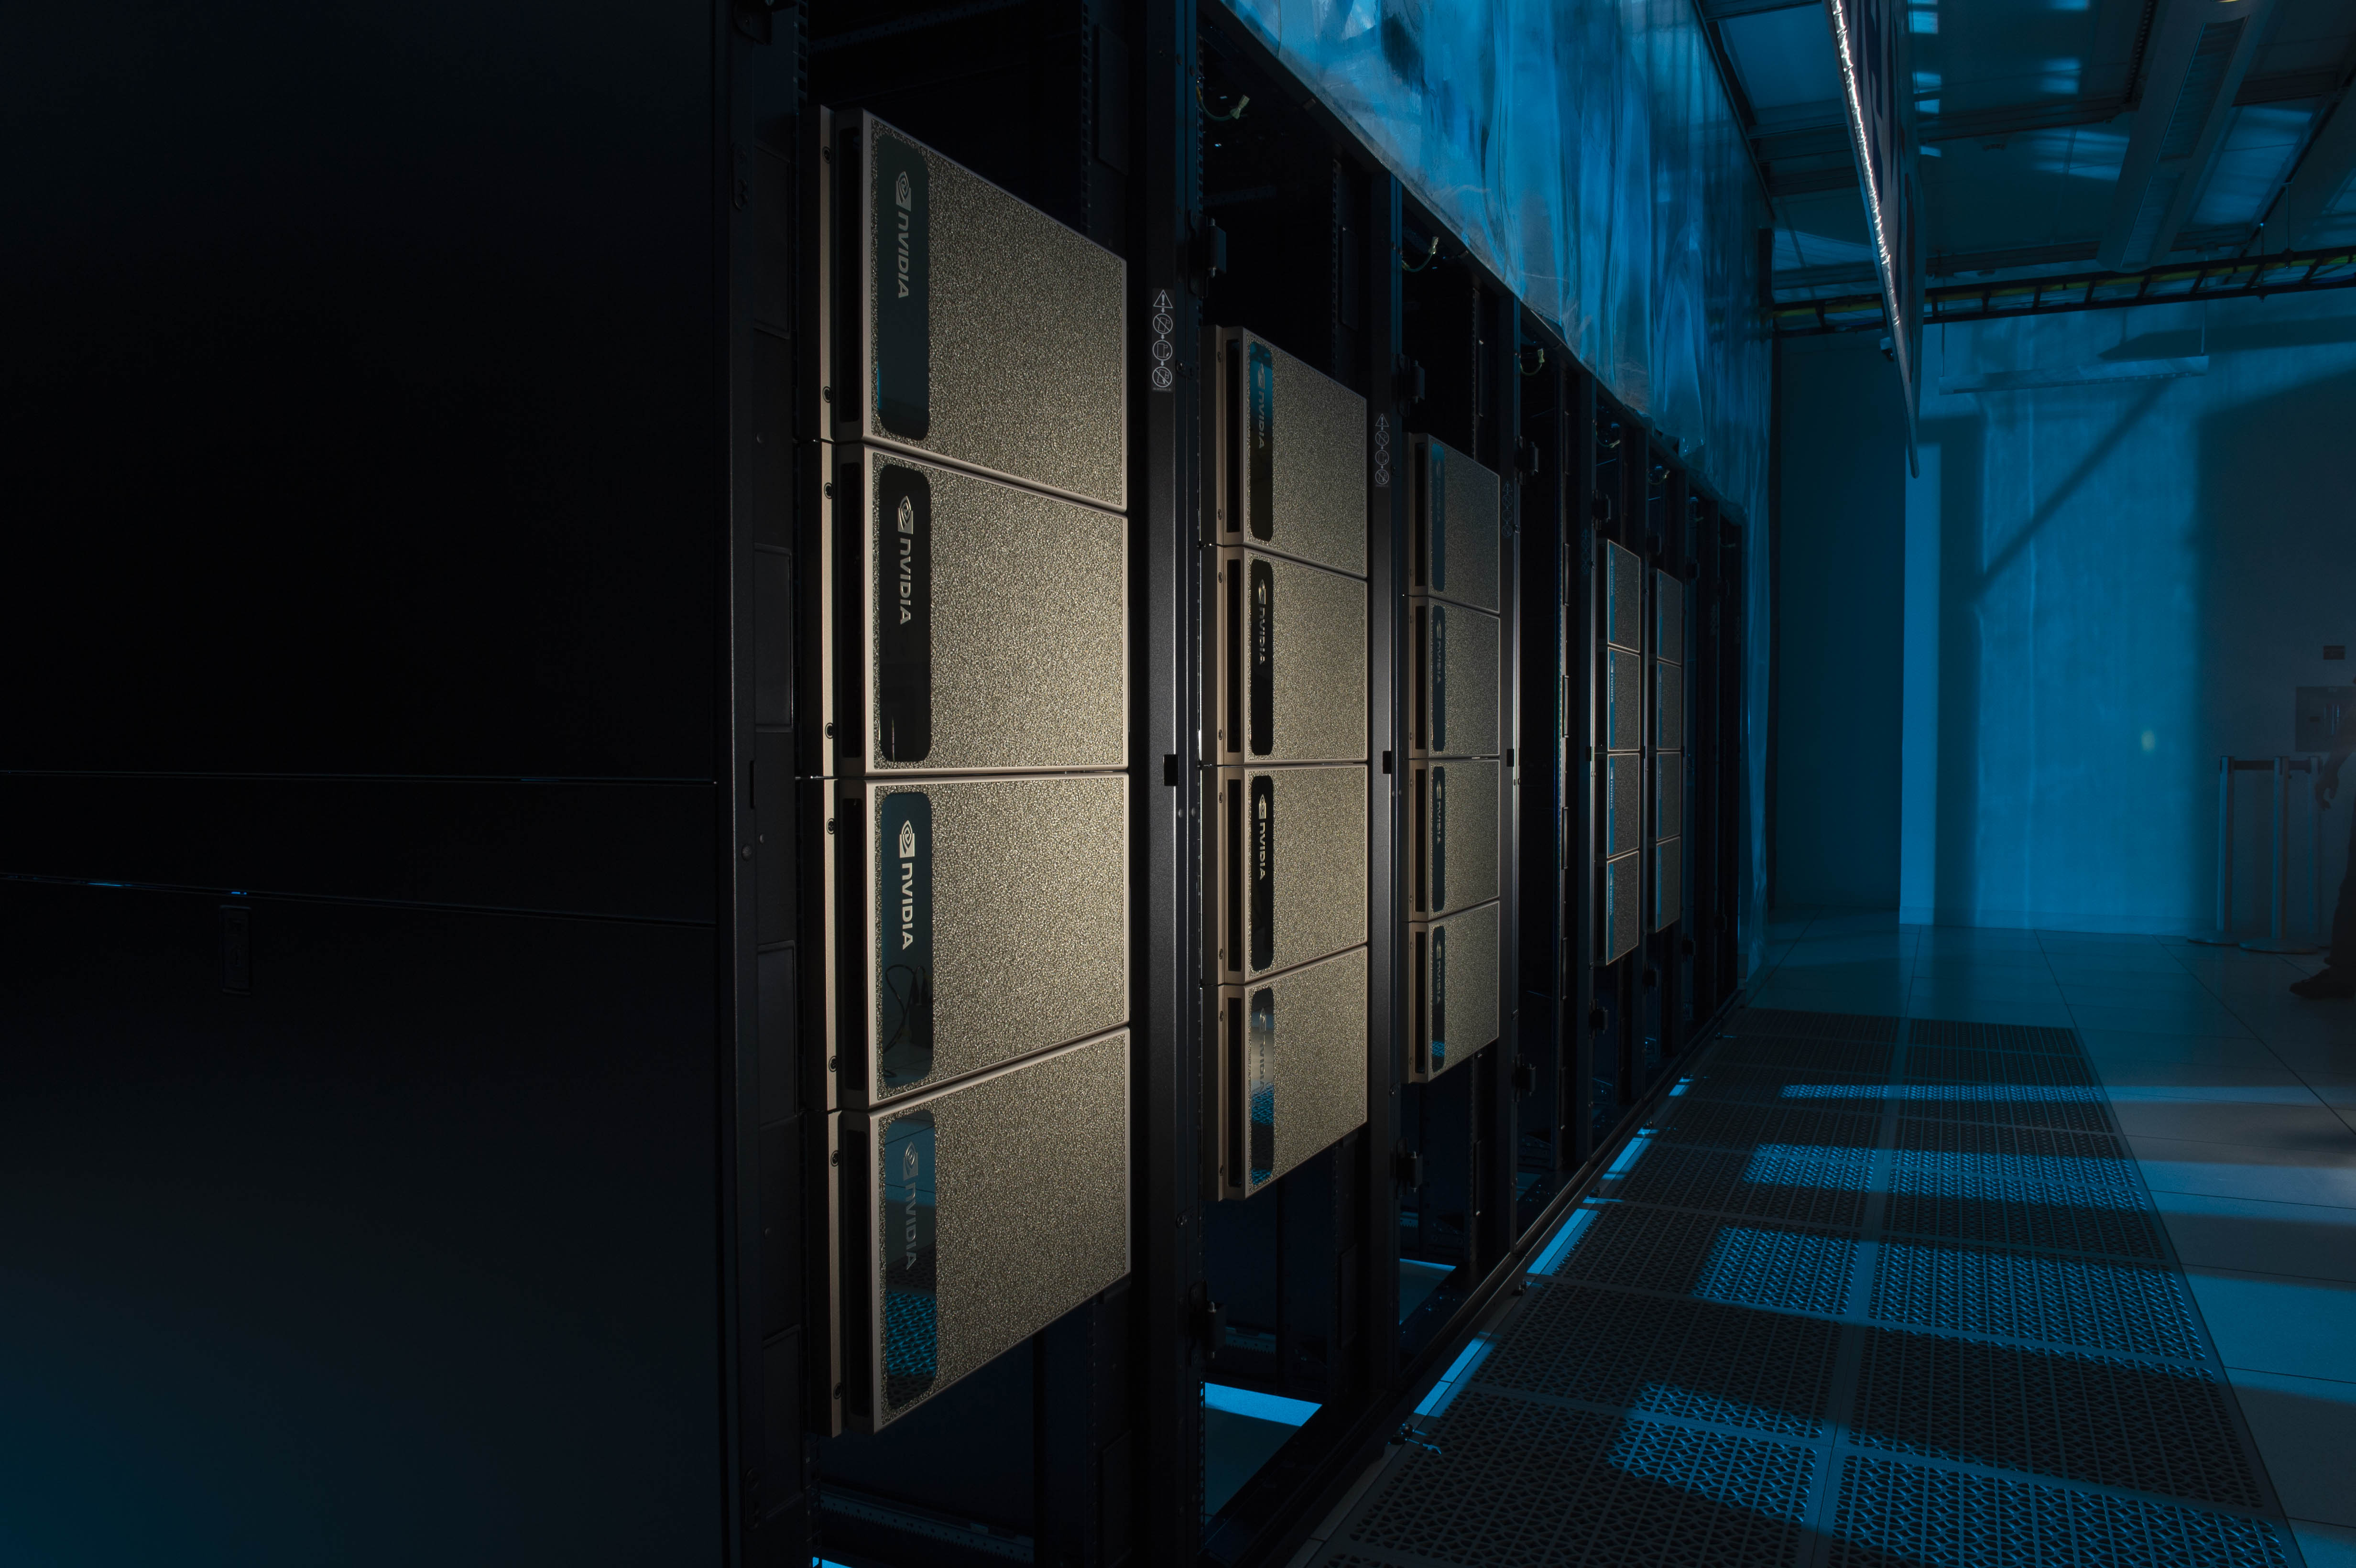
\includegraphics[width=\textwidth]{figures/superpod.jpg}
\end{center}
\end{column}
\end{columns}
\end{frame}

\begin{frame}{SMU HPC File Systems}
\begin{description}
\item[\$HOME]
\begin{itemize}
  \item Default file system when logging into M2, e.g. \mintinline{sh}{/users/$USER}.
  \item Space should be used to write, edit, compile programs, and job submission scripts, etc.
  \item Restricted by quotas (200 GB) and backed-up.
\end{itemize}
\item[\$WORK]
\begin{itemize}
  \item Long term storage at \mintinline{sh}{/work/users/$USER}.
  \item Restricted by quotas (8 TB) and not backed-up.
\end{itemize}
\item[\$SCRATCH]
\begin{itemize}
 \item Scratch space at \mintinline{sh}{/scratch/users/$USER}.
 \item Treat \$SCRATCH as a volatile file system that is not backed-up.
\end{itemize}
\end{description}
\end{frame}

%\begin{frame}{Unversity Data Center (UDC)}
%\begin{columns}
%\begin{column}{0.5\textwidth}
%\begin{center}
%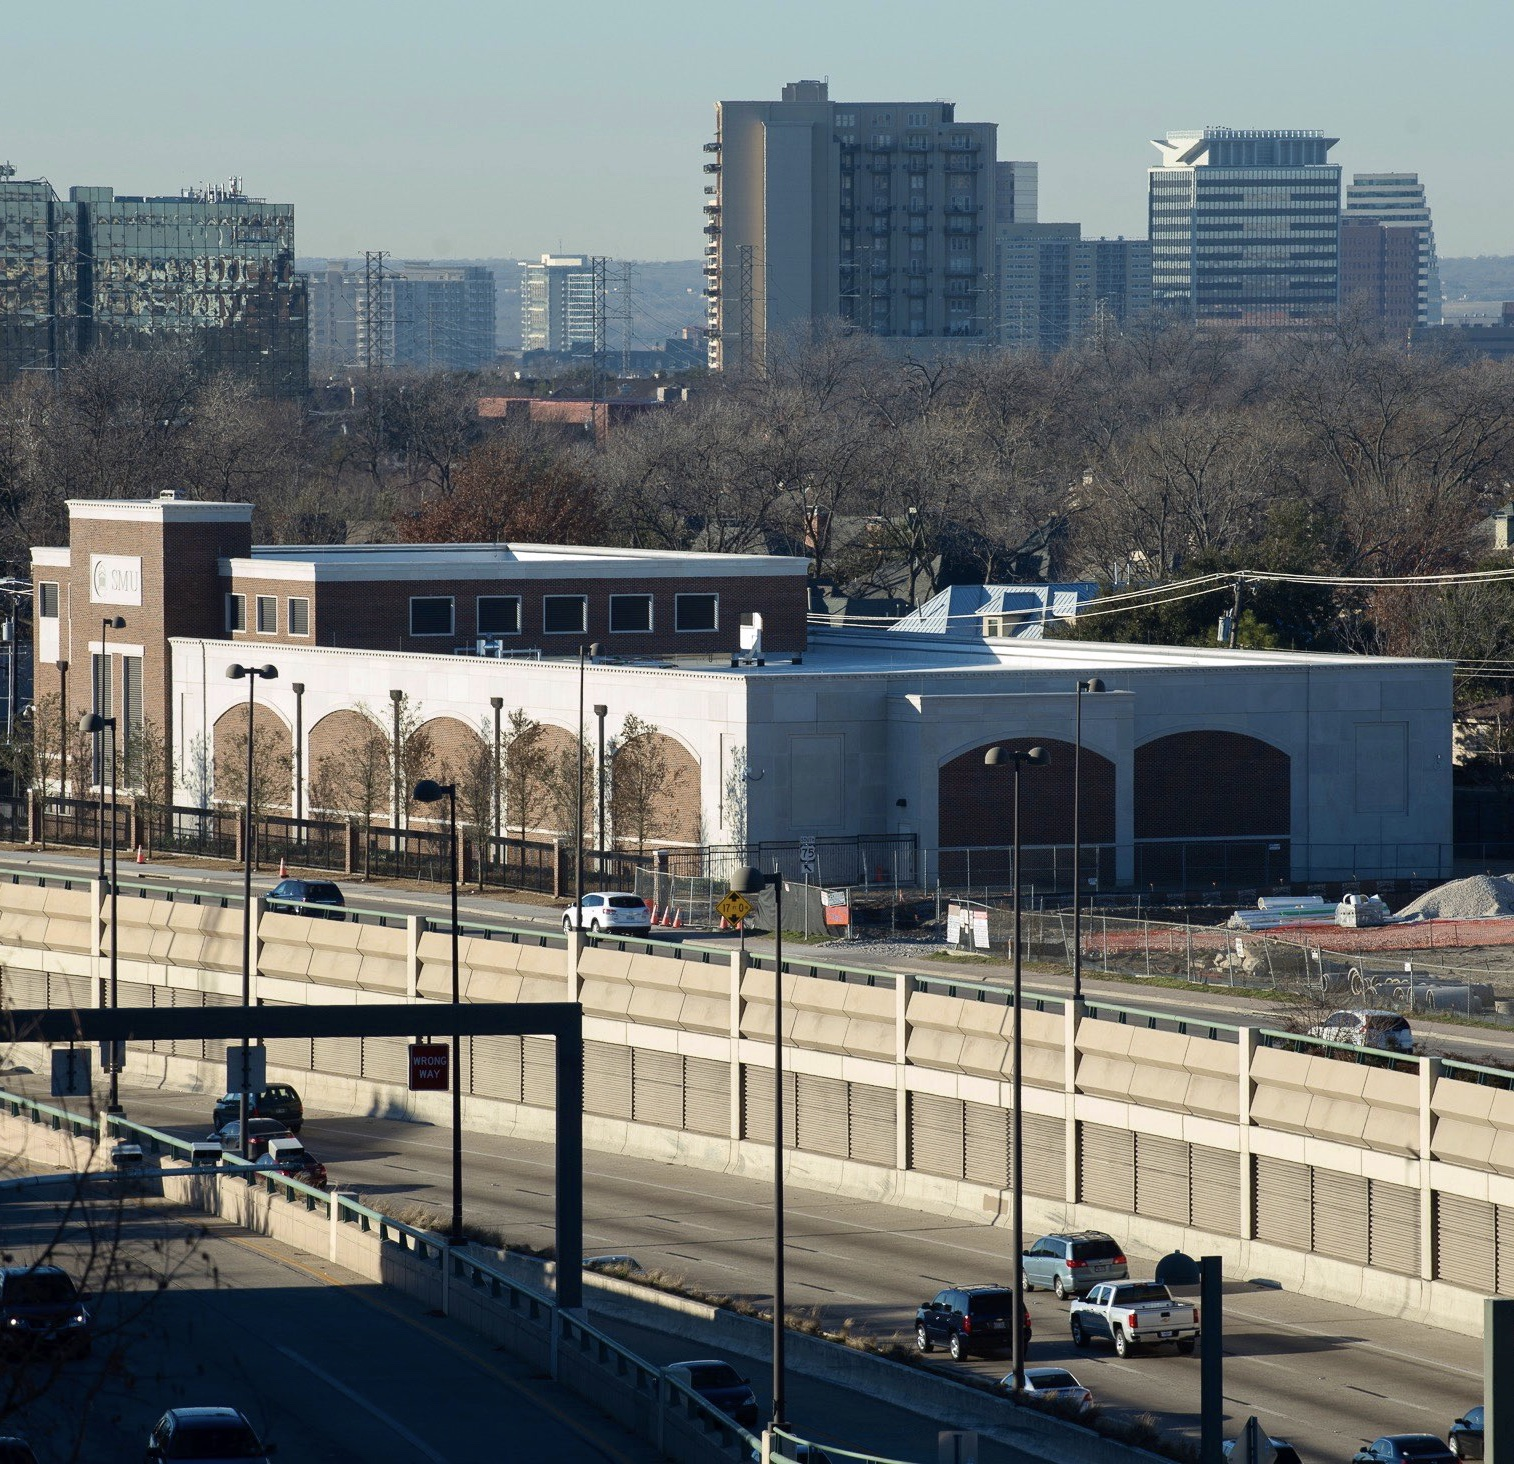
\includegraphics[width=\textwidth]{figures/udc_1.jpg}
%\end{center}
%\end{column}
%\begin{column}{0.5\textwidth}
%\begin{center}
%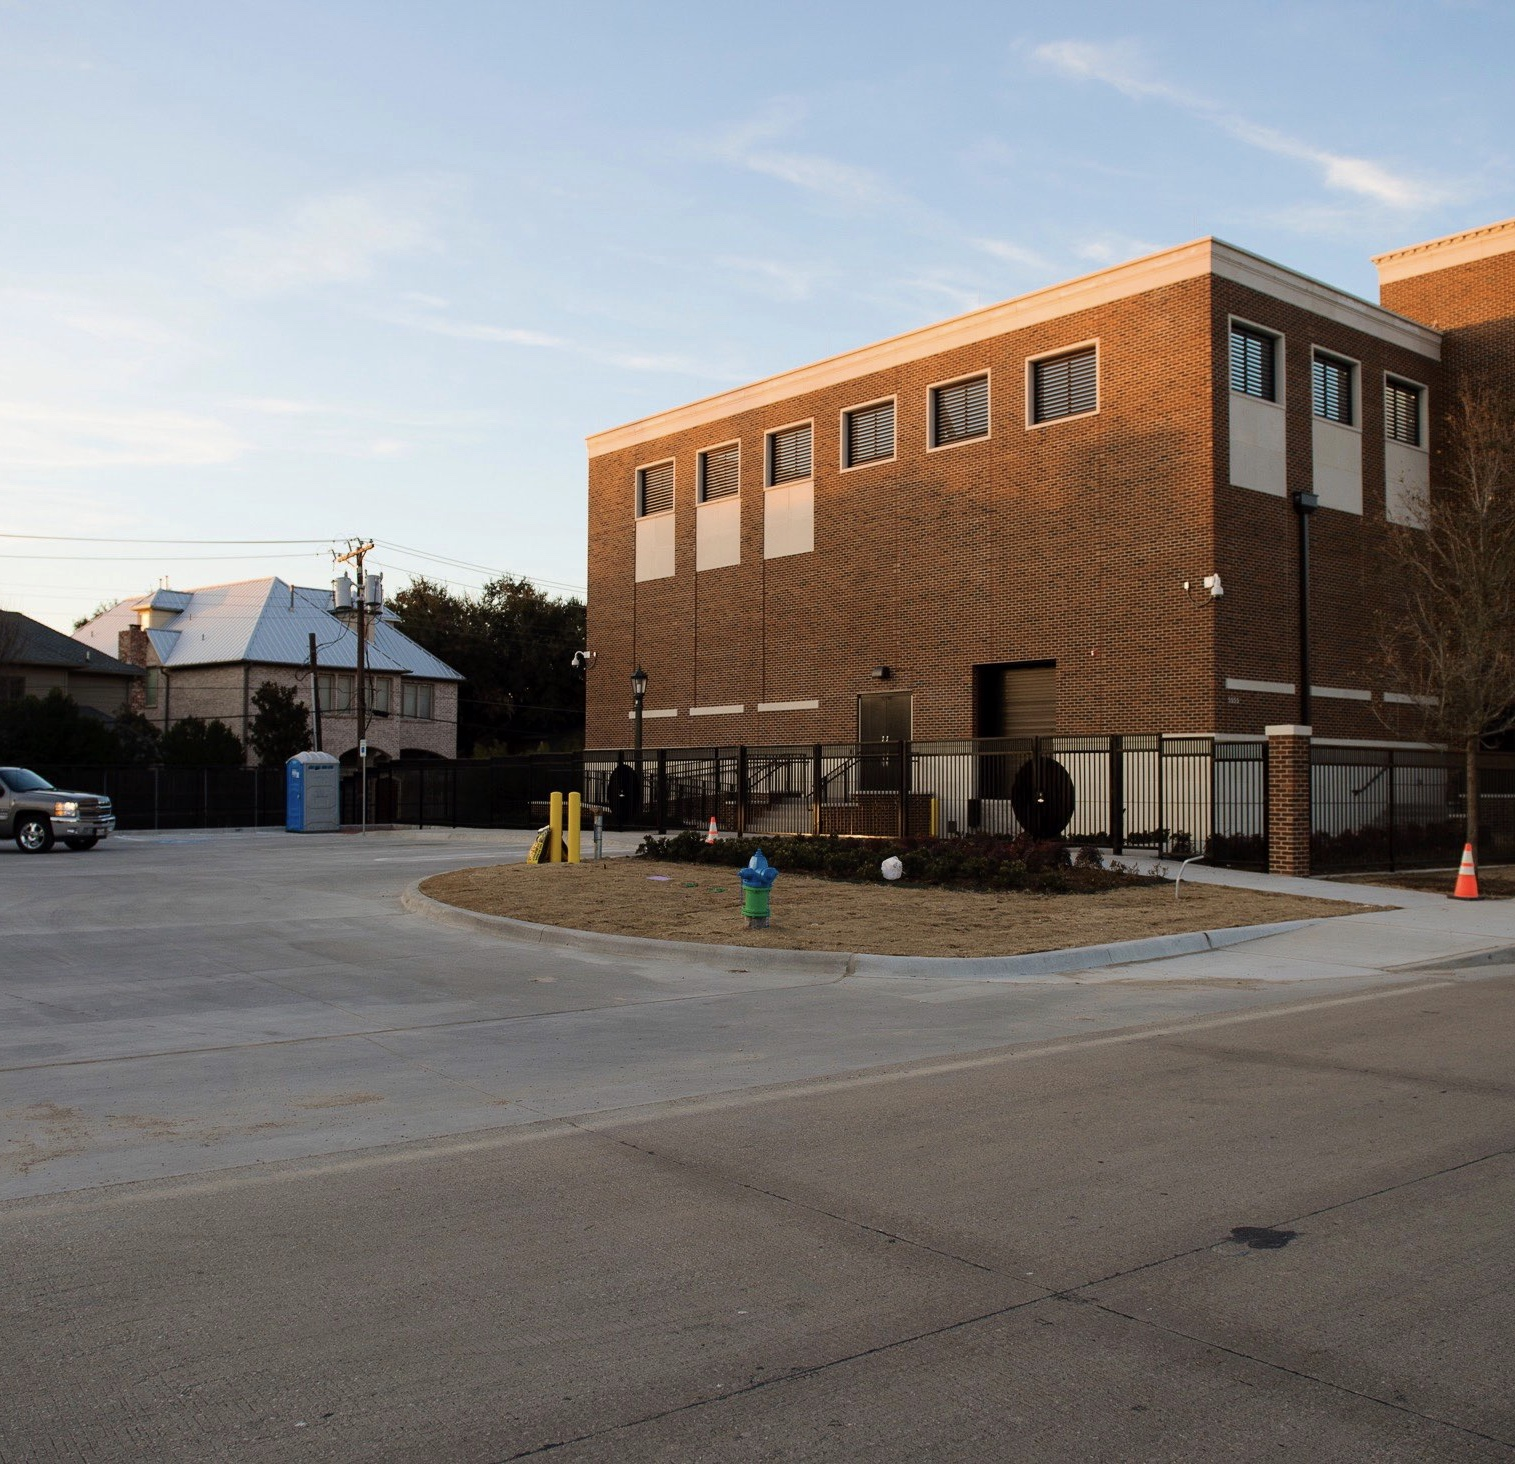
\includegraphics[width=\textwidth]{figures/udc_2.jpg}
%\end{center}
%\end{column}
%\end{columns}
%\end{frame}
%
%\begin{frame}{ManeFrame II (M2)}
%\begin{columns}
%\begin{column}{0.5\textwidth}
%\begin{center}
%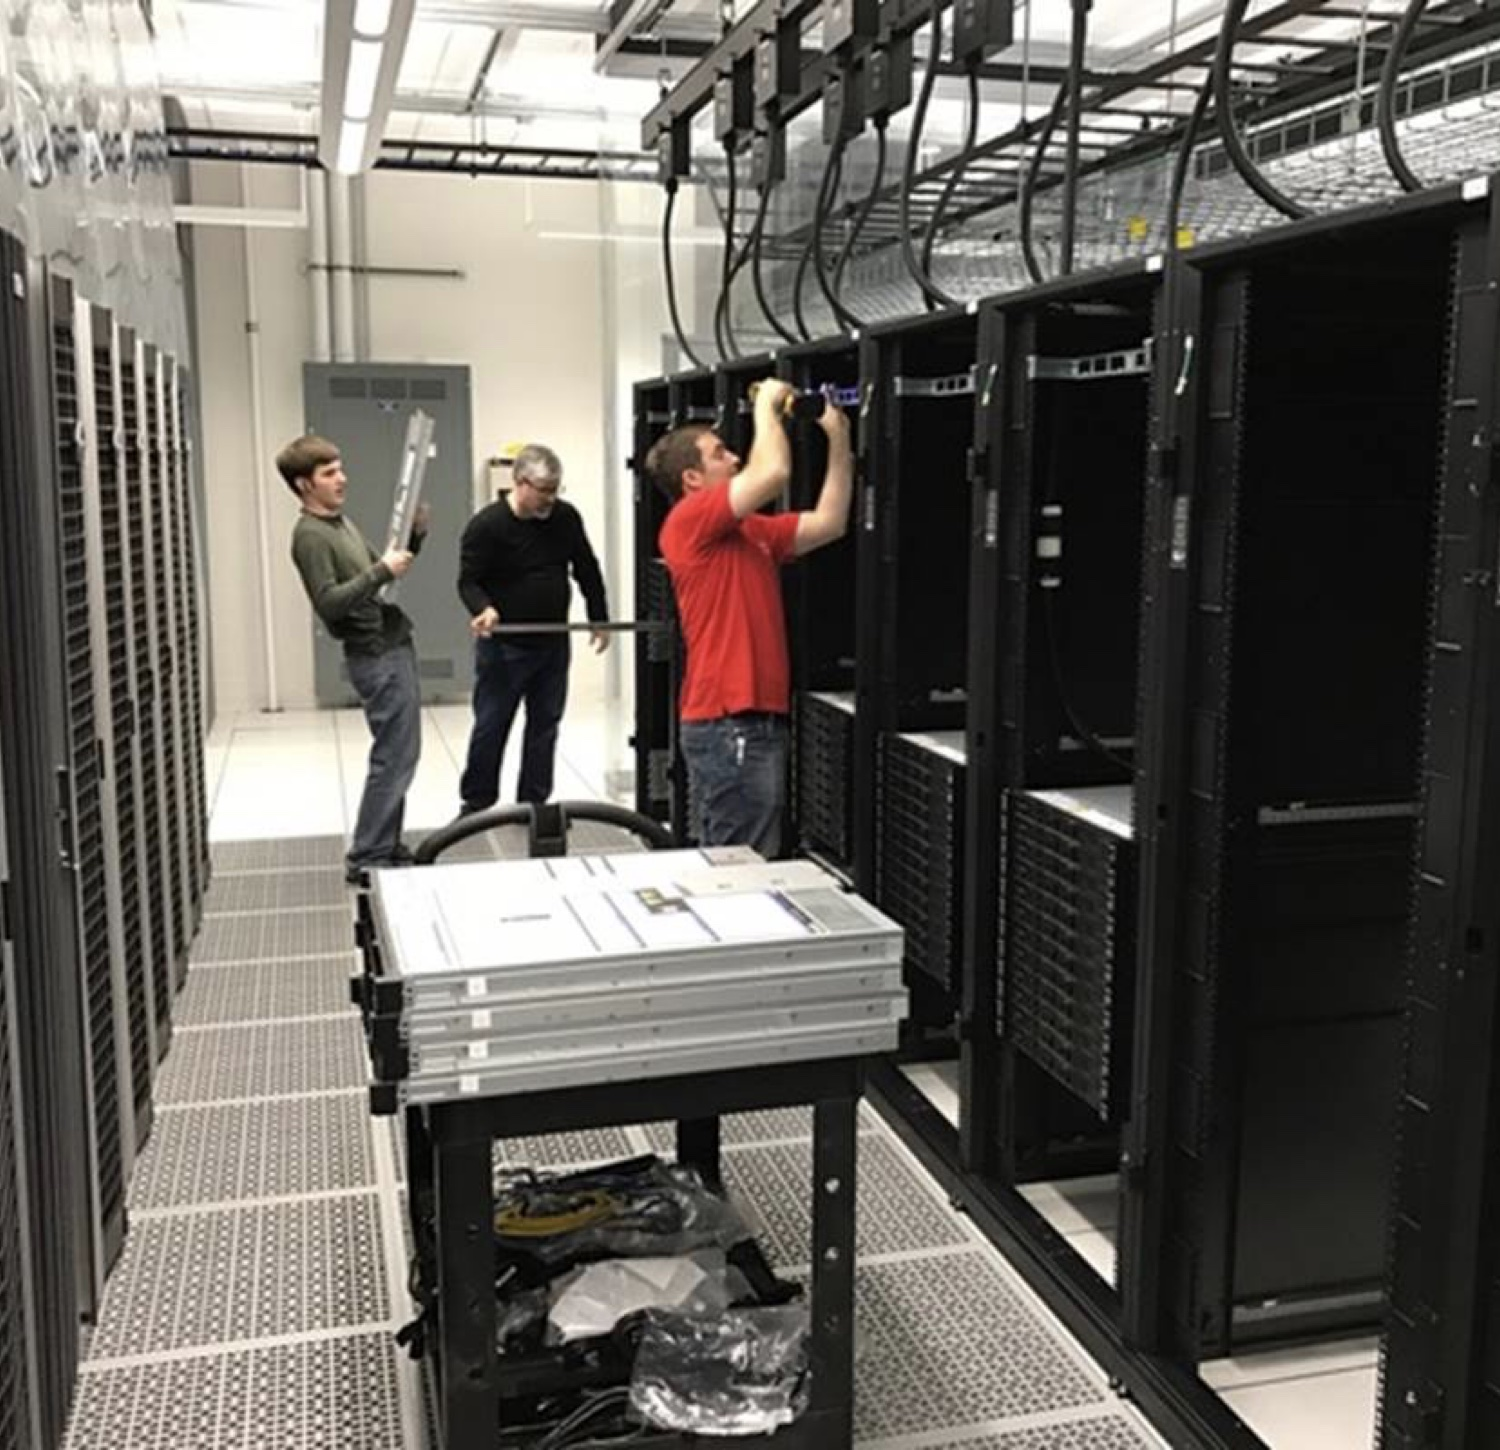
\includegraphics[width=\textwidth]{figures/m2_1.jpg}
%\end{center}
%\end{column}
%\begin{column}{0.5\textwidth}
%\begin{center}
%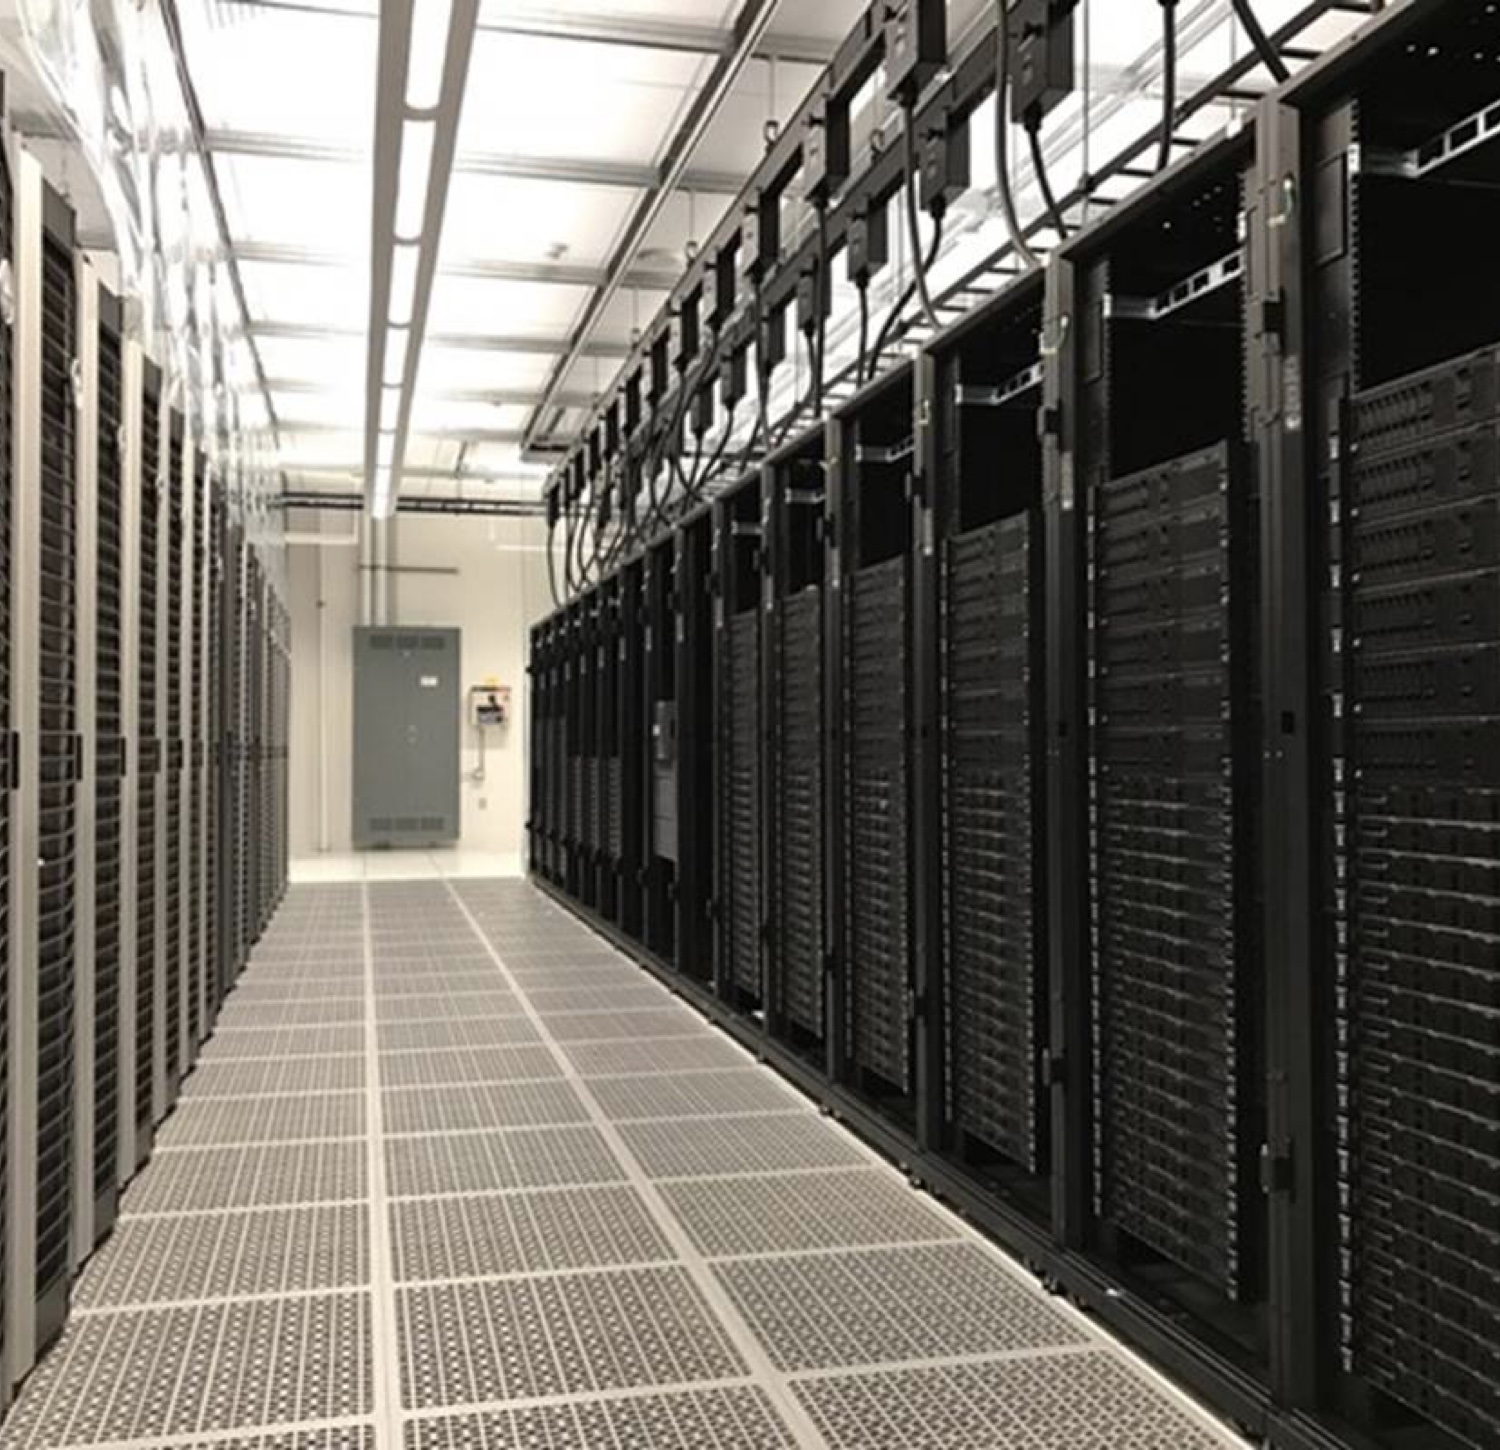
\includegraphics[width=\textwidth]{figures/m2_2.jpg}
%\end{center}
%\end{column}
%\end{columns}
%\end{frame}
%
%\begin{frame}{Hot Aisle Containment}
%\begin{columns}
%\begin{column}{0.5\textwidth}
%\begin{center}
%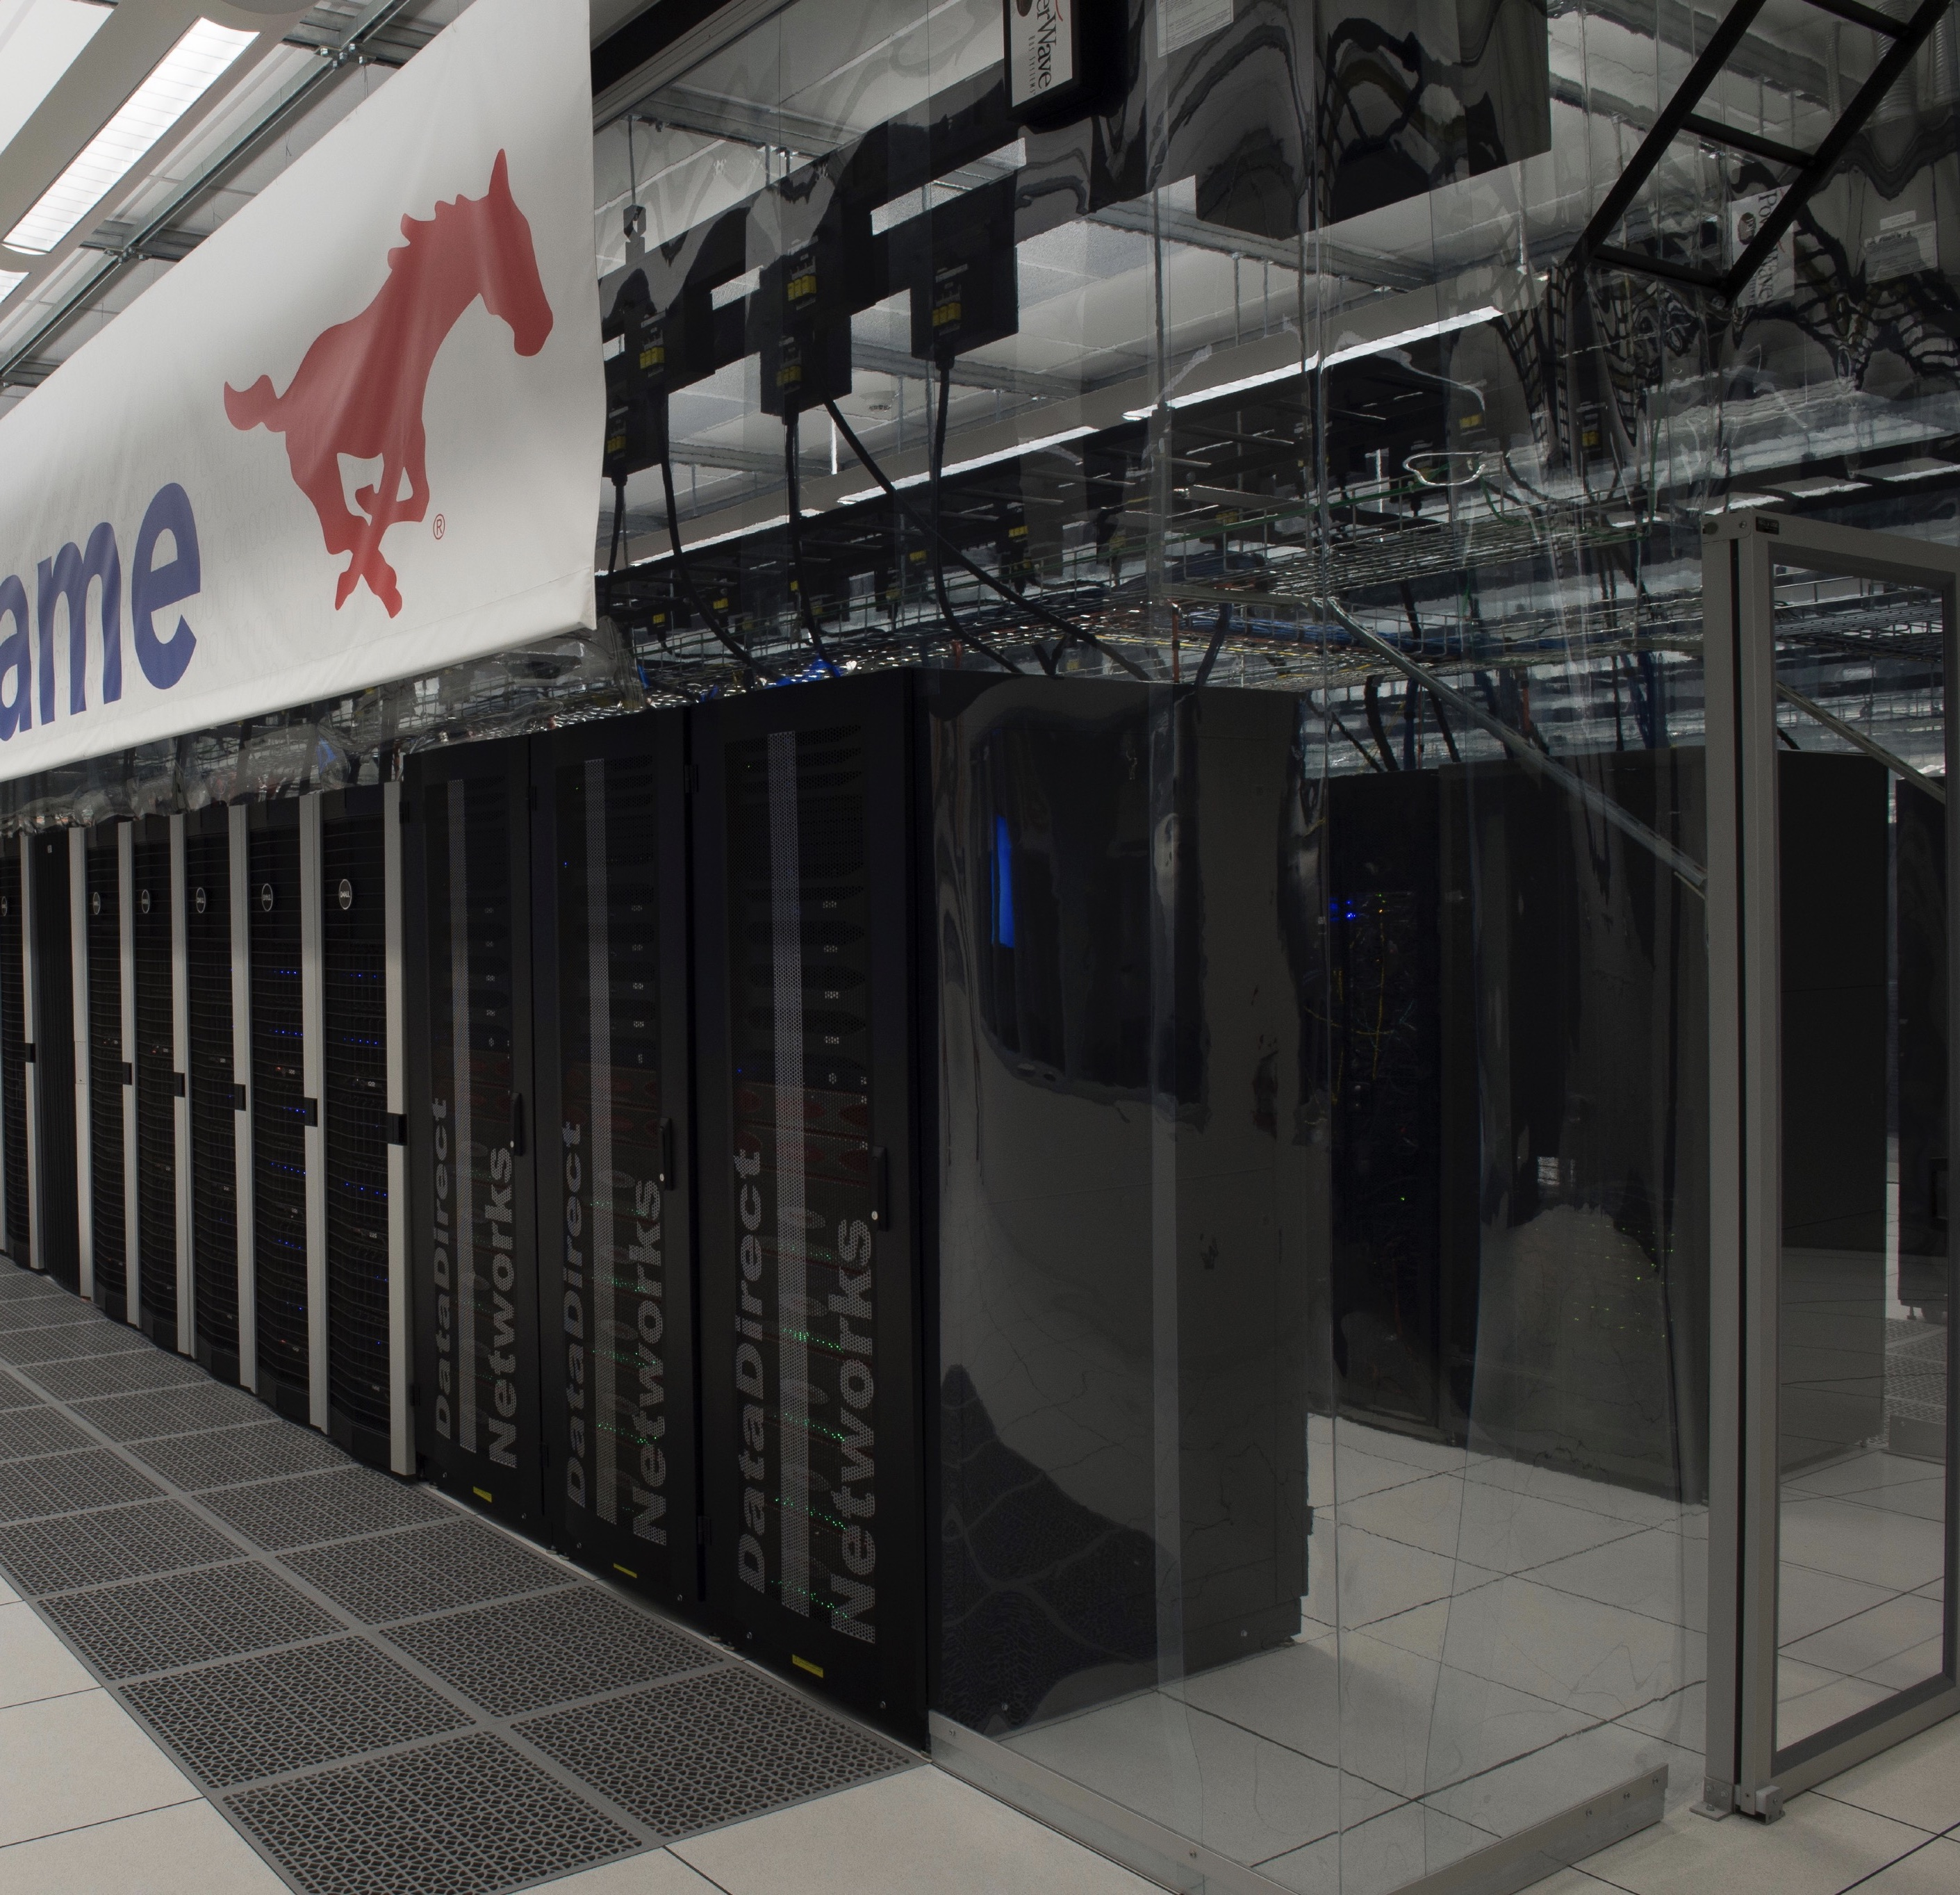
\includegraphics[width=\textwidth]{figures/hot_aisle_1.jpg}
%\end{center}
%\end{column}
%\begin{column}{0.5\textwidth}
%\begin{center}
%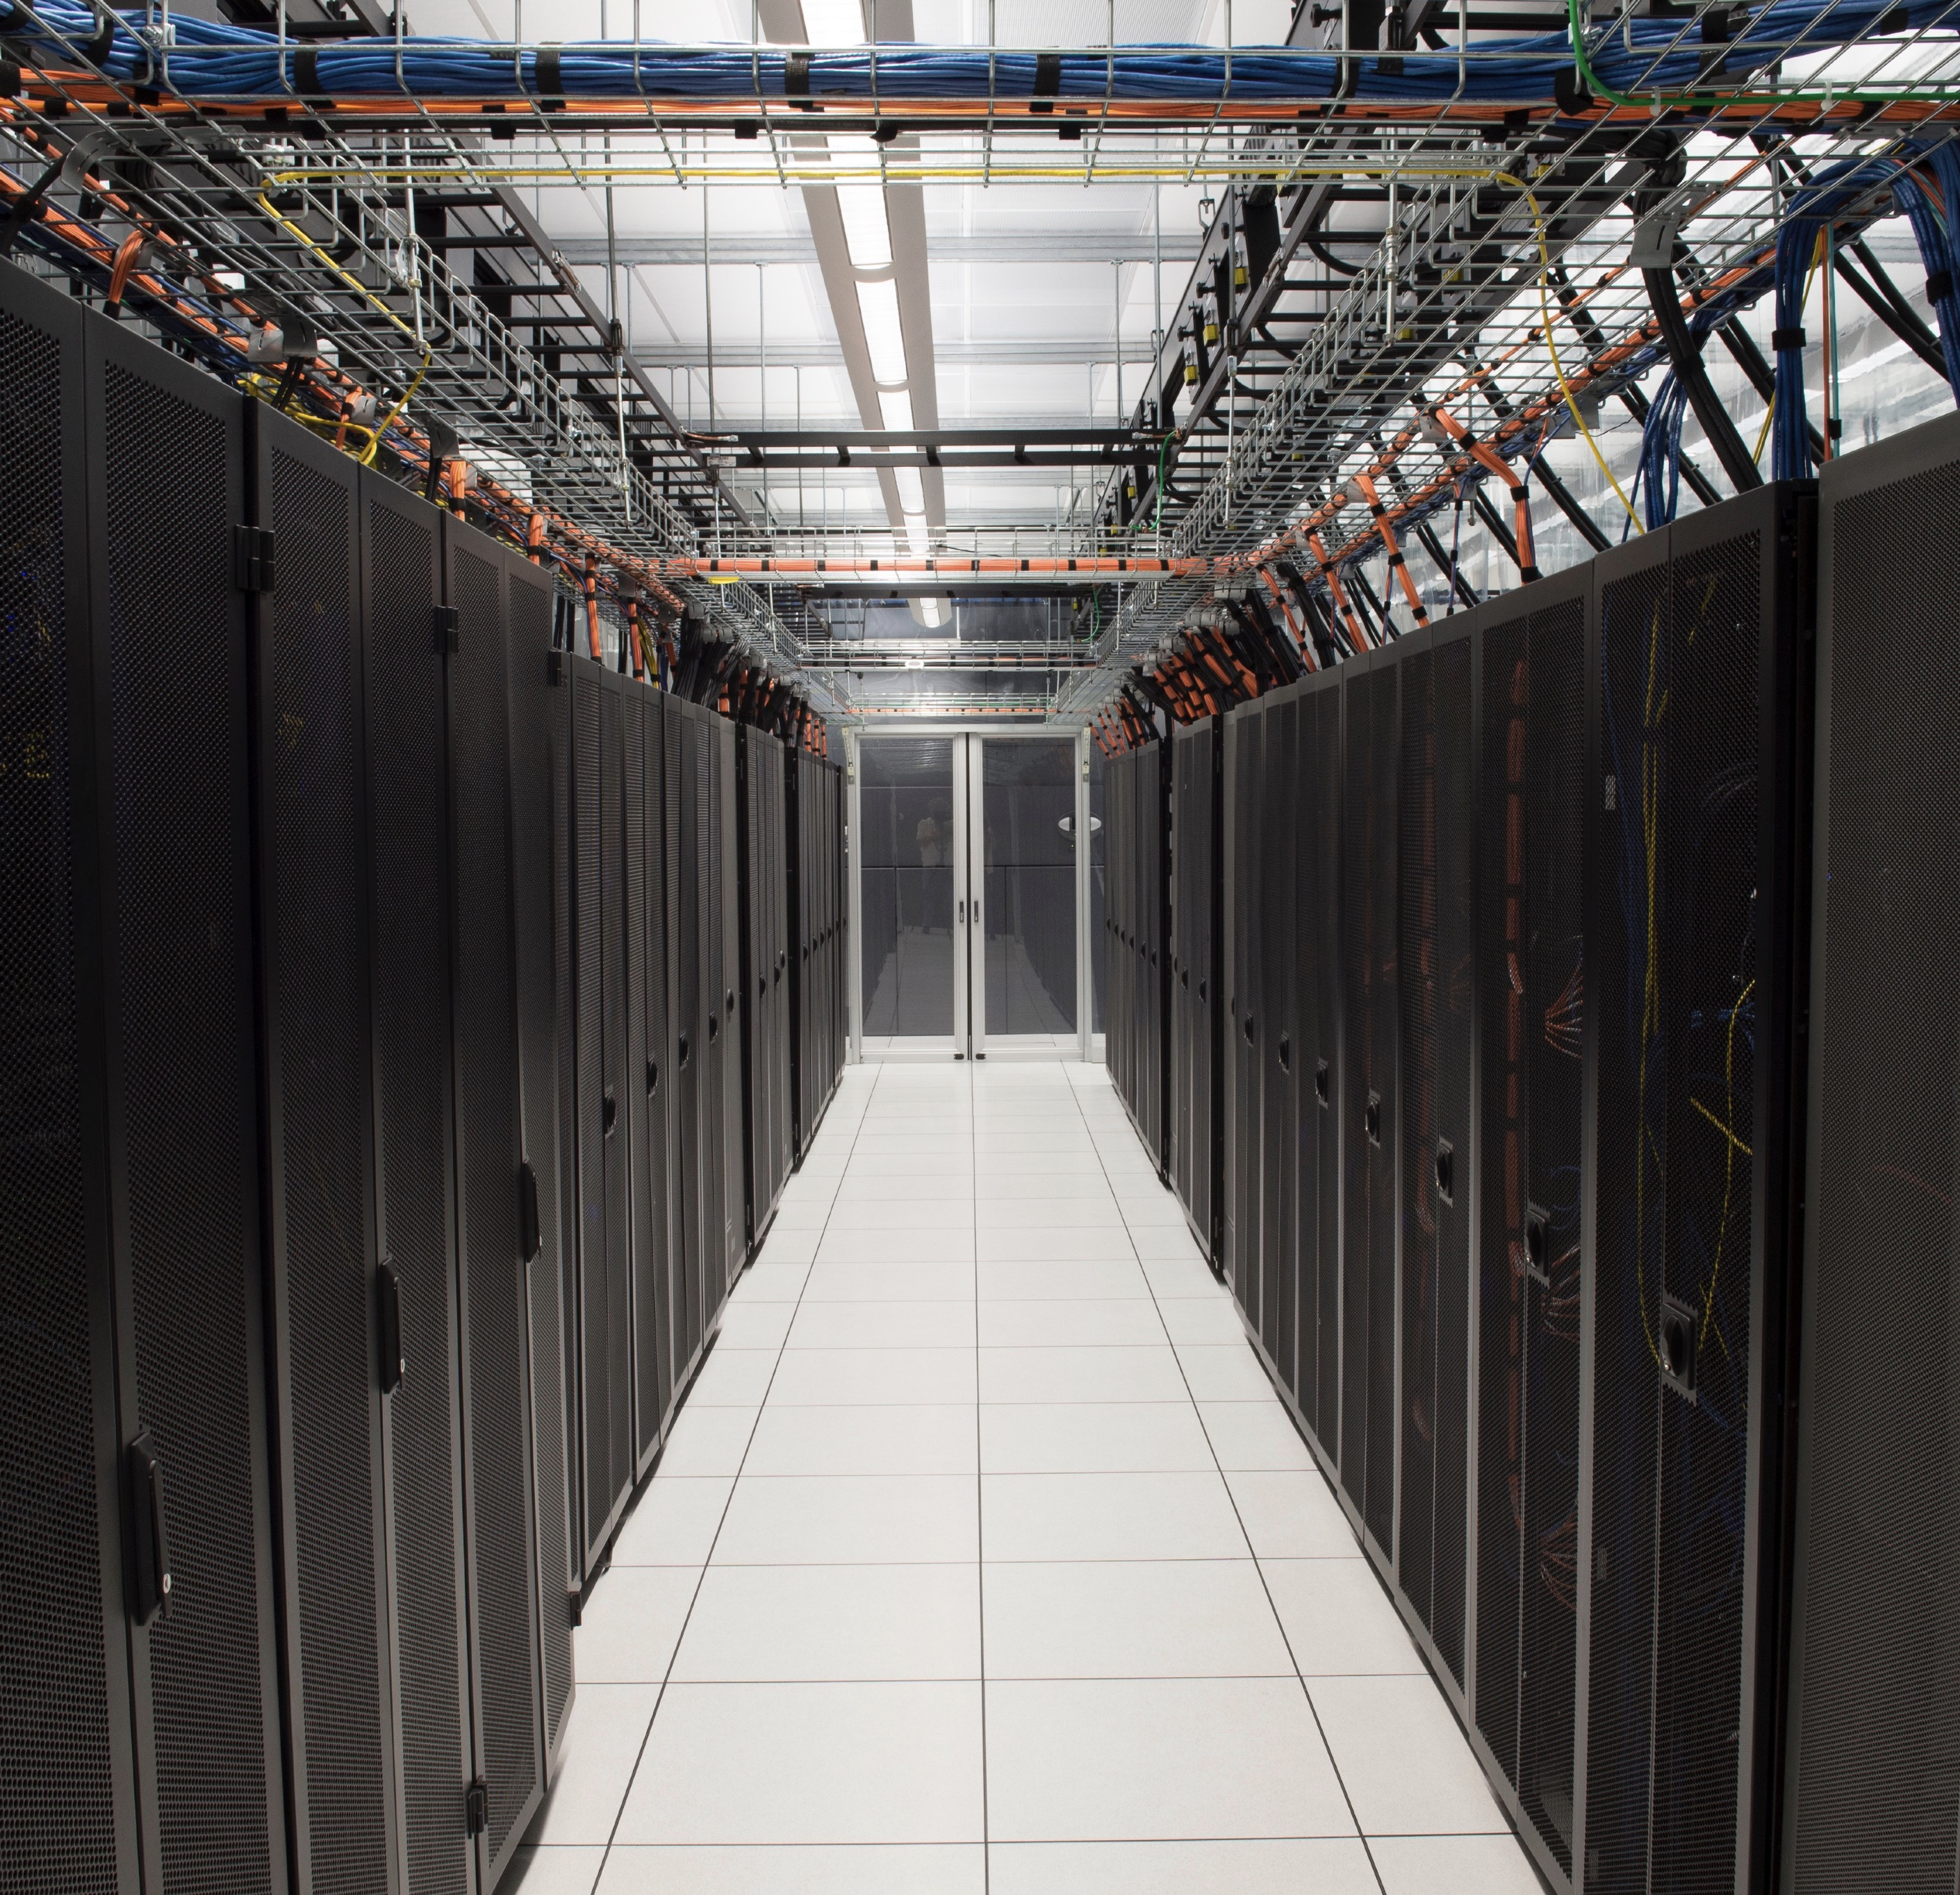
\includegraphics[width=\textwidth]{figures/hot_aisle_2.jpg}
%\end{center}
%\end{column}
%\end{columns}
%\end{frame}
%
%\begin{frame}{Cooling and Power}
%\begin{columns}
%\begin{column}{0.5\textwidth}
%\begin{center}
%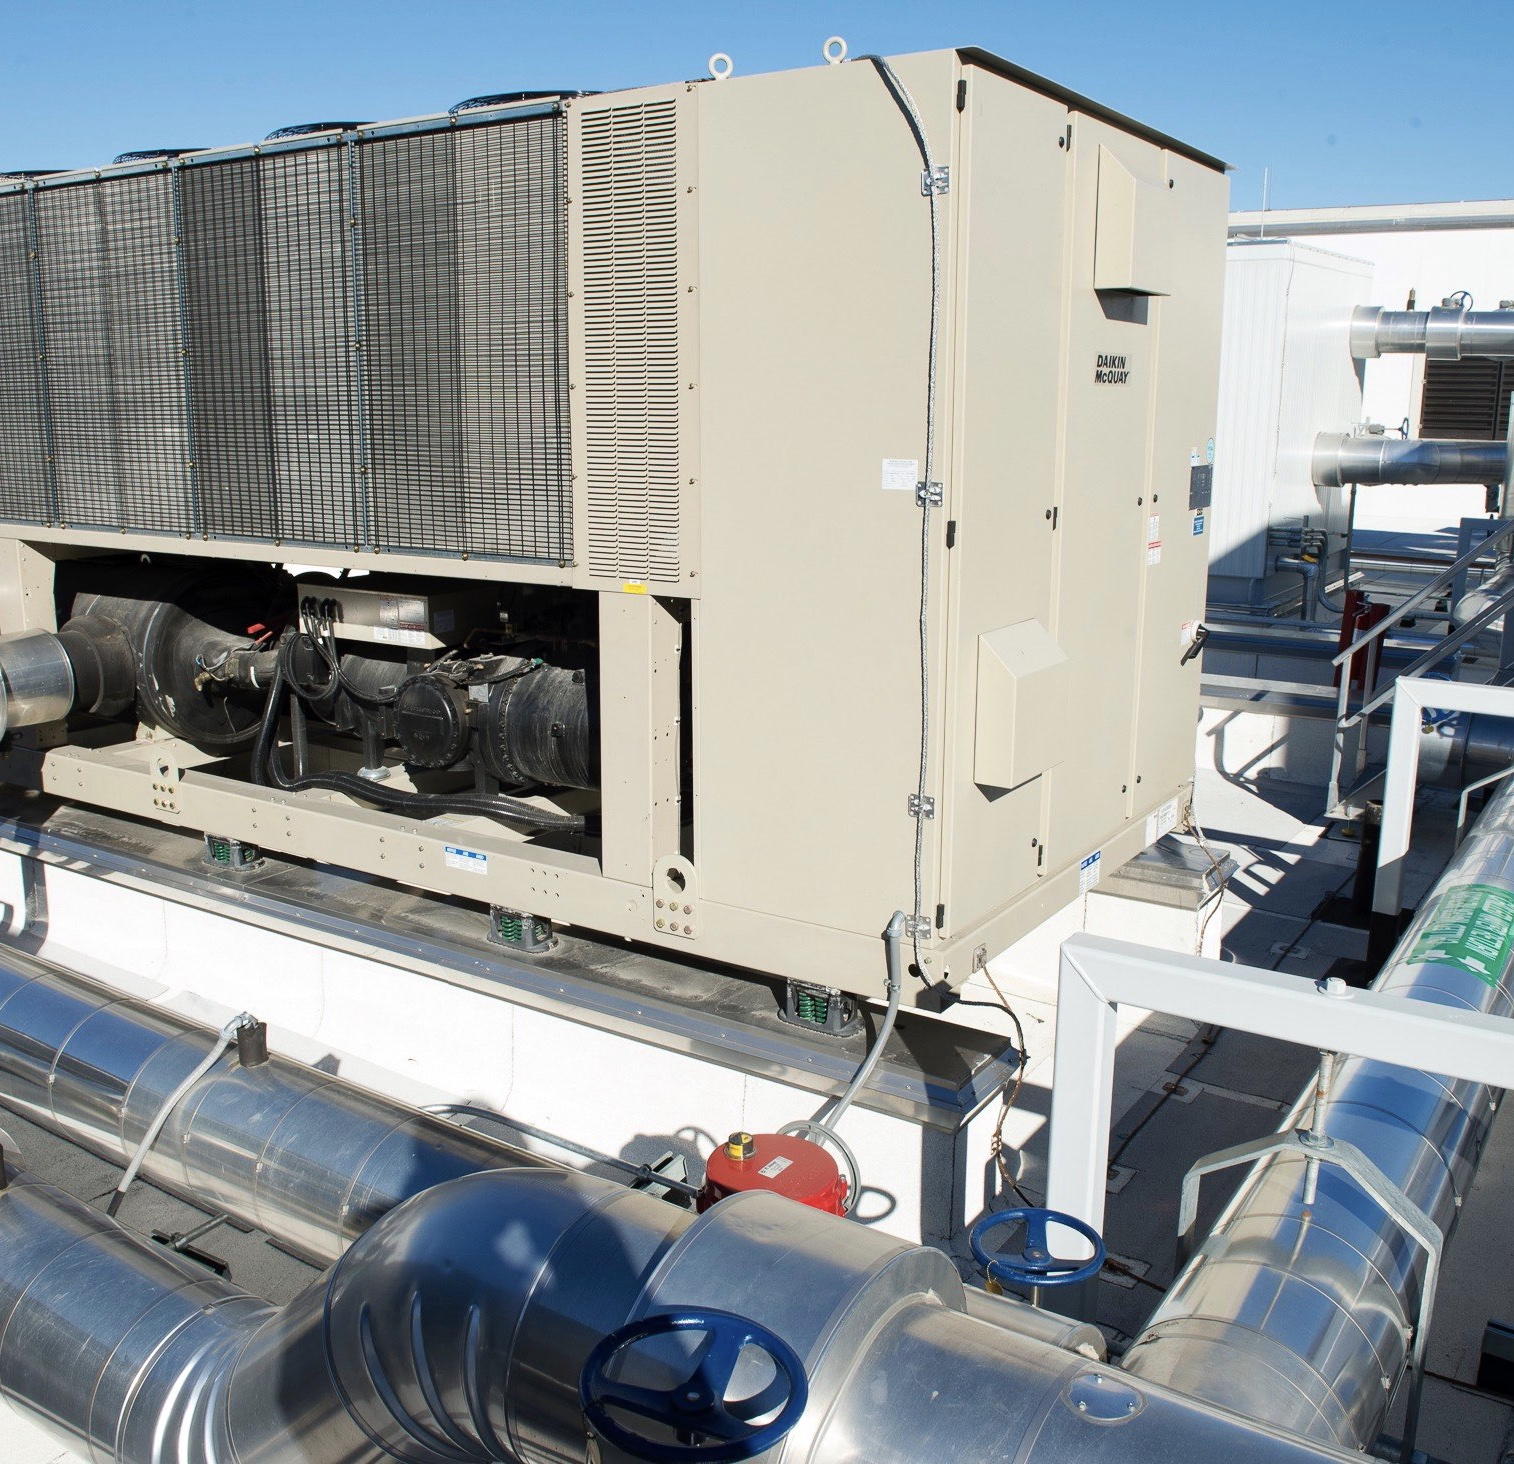
\includegraphics[width=\textwidth]{figures/cooling.jpg}
%\end{center}
%\end{column}
%\begin{column}{0.5\textwidth}
%\begin{center}
%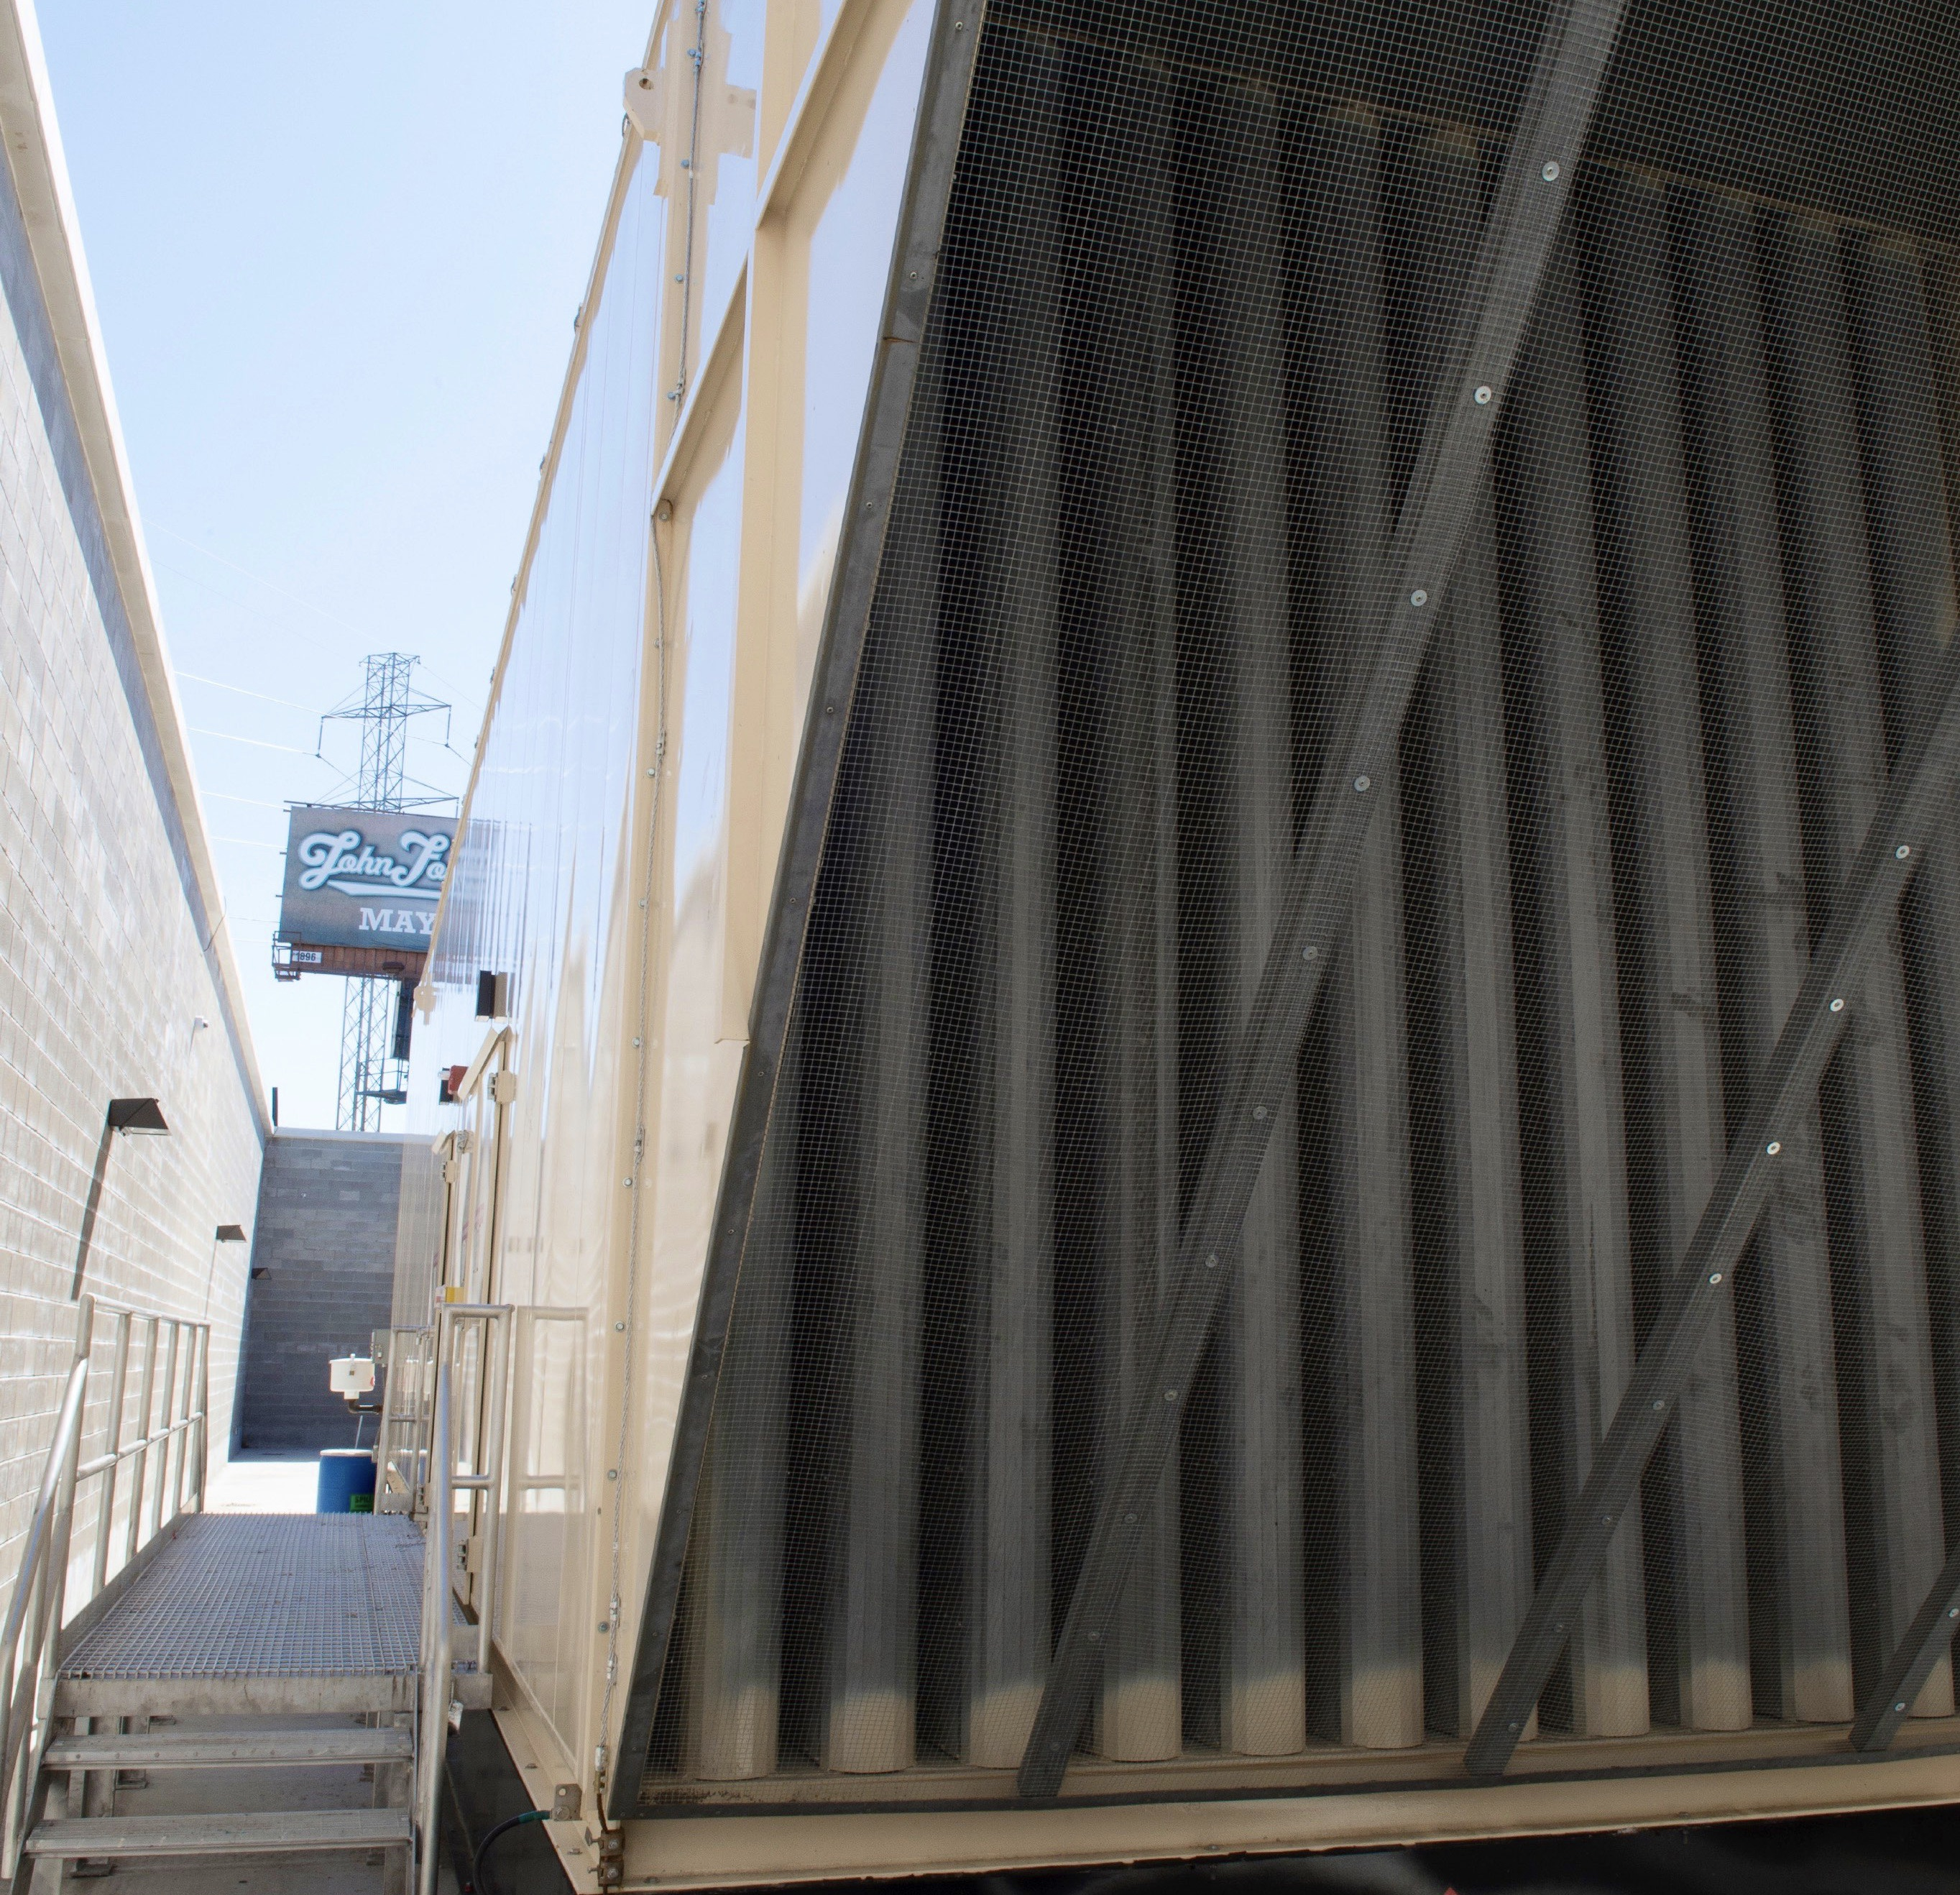
\includegraphics[width=\textwidth]{figures/power.jpg}
%\end{center}
%\end{column}
%\end{columns}
%\end{frame}

